
\chapter{Prestatieverwachtingen}
\label{Prestatie_verwachtingen}
\textit{In dit hoofdstuk worden de prestaties verwachtingen toegelicht aan de hand van de in \cref{cha:opdrachtanalyse} opgestelde prestatie criteria (\cref{se:PC}) en functionele eisen (\cref{se:PVE}). In \cref{se:presentatie_ontwerp} wordt het ontwikkelde concept gepresenteerd, hier wordt een korte omschrijving van het ontwerp gegeven samen met een afbeelding. In \cref{se:prestatie_en_eigenschappen} worden de verwachte prestaties verteld met eventuele berekeningen om dezen te ondersteunen, ook worden hier de specifieke eigenschappen van het ontwerp toegelicht. In \cref{se:veiligheidsanalyse_prestatieverwachting} wordt een veiligheid-overzicht van het ontwerp gepresenteerd.}

\section{Presentatie van het ontwerp}
\label{se:presentatie_ontwerp}

De Driepoter is een ontwerp dat in staat is om over obstakels heen te stappen door middel van zijn inklapbare poten. Zoals te zien is in \cref{fig:De_driepoter_Prestatie_analyse} is de Driepoter in staat om de schaarliften die hij aan de onderkant van het chassis heeft in te klappen en uit te klappen. De Driepoter kan het pakket ontvangen door middel van een rol-baar plateau, dit zorgt ervoor dat de Drieklapper een verstelbaar zwaarte punt heeft wat handig is voor het nemen van een talud. Eenmaal wanneer de Driepoter een bocht moet maken kan hij zien voorste wielen draaien en net als een auto een bocht maken.\\

\vspace{\baselineskip}
\begin{figure}[H]
    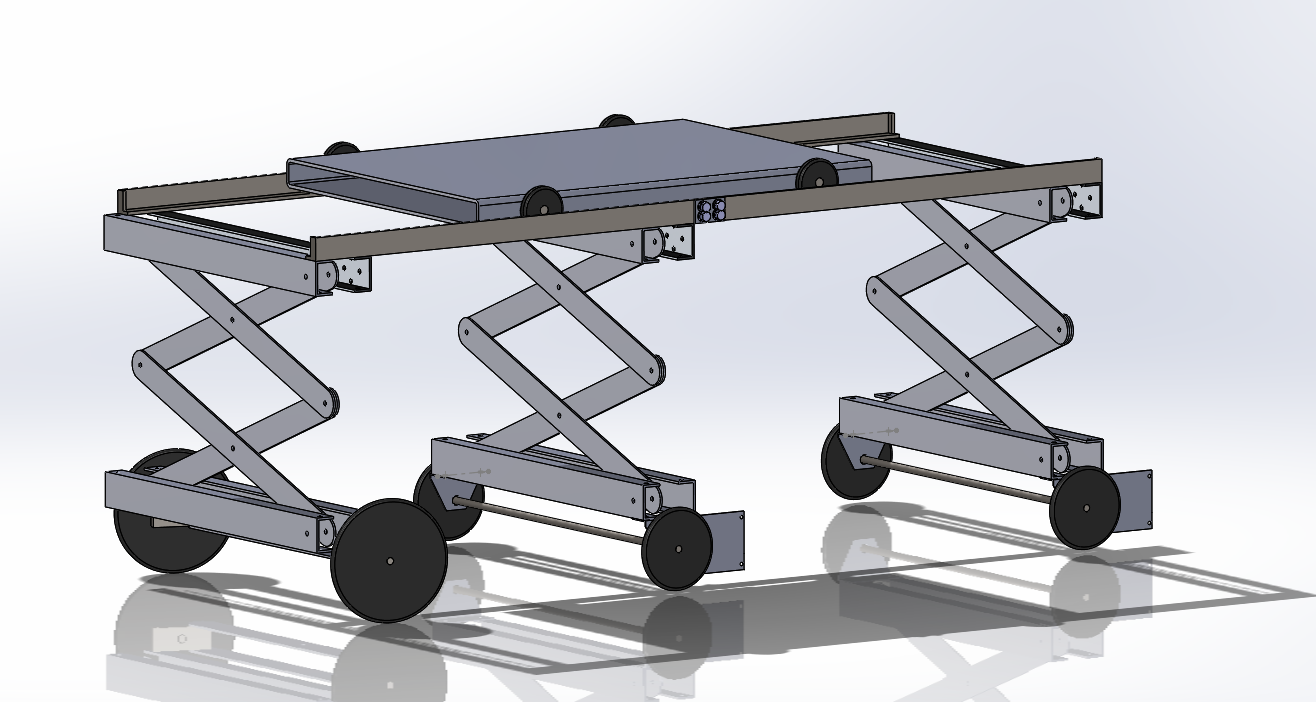
\includegraphics[width = 120mm]{04_gekozenconcept/eindconcept.png}
    \caption{de Driepoter}
    \label{fig:De_driepoter_Prestatie_analyse}
\end{figure}


\section{Verwachte eigenschappen en prestaties}
\label{se:prestatie_en_eigenschappen}
Hier worden de prestaties en de eigenschappen van de Driepoter besproken en onderbouwt door middel van berekeningen en bronnen. De mogelijke prestaties zijn aan de hand van de prestatie criteria en het programma van eisen in \cref{cha:opdrachtanalyse} opgesteld. De gekozen prestaties en eigenschappen die moet worden bepaald zijn: De dynamische en statische stabiliteit, het balans van het pakketje, de benodigde hoeveelheid energie voor het nemen van de hindernis baan en de tijd die het pakket hondje kost voor het nemen van de hindernisbaan. 

\subsection{De stabiliteit}
Erg belangrijk is het voor het pakkethondje dat hij niet omvalt tijdens het versnellen, afremmen of het nemen van een talud. De stabiliteit is in twee delen verdeeld: de dynamische stabiliteit en de statische stabiliteit. Onder de dynamische stabiliteit valt het versnellen en remmen van het pakkethondje en onder de statische stabiliteit valt het nemen van een talud en het rijden van het pakkethondje.\\
Voordat er berekeningen worden gedaan moeten een aantal parameters worden bepaalt:

\begin{itemize}

    \item \textbf{De hoogte van het massamiddelpunt bij verschillende tijdstippen in het nemen van de hindernisbaan}. De formule voor de hoogte van het massa middelpunt is bepaald in \cref{se:Bijlage_H_mmp}.\\
    Als de juiste parameters worden ingevuld worden de volgende hoogtes bij de volgende situaties bepaald:\\
    \textit{\textbf{h1} = 0,17 m,  hoogte van het massamiddelpunt tijdens het rijden\\
    \textbf{h2} = 0,45 m,  hoogte van het massamiddelpunt tijdens het ontvangen van het pakket \\
    \textbf{h3} = 0,63 m, de hoogte van het massamiddelpunt tijdens het nemen van talud 2\\}

    \item \textbf{Het steunvlak}. Deze wordt bepaald door de 3 paar wielen aan de onderkant van de schaarlift. De wielen staan 530 mm en 350mm van elkaar af. Hieruit kan worden berekend met een simpele rekensom wat de steunvlakken zijn bij de verschillende situaties. \textit{Tijdens het rijden is het steunvlak 530 x 700 mm} en \textit{tijdens het nemen van het talud is het steunvlak 530 x 350 mm}
    
    \item \textbf{Eventuele externe krachten of veranderingen in deze krachten.} De verwachting is dat de wind en de andere externe krachten minimaal zullen zijn. Wel moet er eventueel rekening worden gehouden met de klinker waarop het pakkethondje rijdt. Er moet worden bepaald hoe scheef het pakkethondje kan gaan staan door toe doen van de klinkers zodat hij niet kantel tijdens het rijden.\\
    Er is niet een precieze waarde te vinden dus de inschatting is dat een klinker ongeveer maximaal 3 cm uit de grond steekt ten opzichte de 'kuiltjes' die zich tussen de klinkers bevinden. Dit zorgt ervoor dat het pakkethondje scheef zou kunnen staan met een hoek van \textit{3,2 \textdegree.}\\
    
    \item \textbf{Maximale hoek van talud 1.} Deze waarde is te gevonden in \cite{beek_2020_wedstrijdregelement}. De maximale hoek van talud 1 is $6,50$ \textdegree.

    \item \textbf{Relevante constanten.} Er is een lijst opgesteld van relevante constanten die te zien is in \cref{se:Bijlage_H_relevante_constanten}.
    
\end{itemize}
\vspace{\baselineskip}

\textbf{Dynamische stabiliteit.}Voor hoe de berekening moest worden opgezet is gebruik gemaakt van \cite{hof_gazendam_sinke_2004}. Dit stelt dat de projectie van de resulterende kracht van de massa x versnelling in horizontale richting en de massa x gravitatie versnelling in de verticale richting voor dynamische stabiliteit binnen het steunvlak moet blijven. Wanneer aan deze voorwaarde voldoet tijdens het versnellen of remmen blijft het pakkethondje overeind. Hier is aan gerekend en de conclusie eruit was de het pakkethondje tijdens het versnellen en afremmen overeind blijft. \\
Uit de berekeningen, te vinden in \cref{se:Bijlage_H_Dynamische_stabiliteit} volgt dat \textit{het pakkethondje overeind blijft staan tijdens het rijden.}\\
\vspace{\baselineskip}

\textbf{Statische stabiliteit.} Ook moet er worden gekeken de statische balans, er moet worden bepaald of het pakket hondje niet om valt tijdens het nemen van het talud.\\
In \cref{se:Bijlage_H_Statische_stabiliteit} is een berekening gemaakt wat betreft de statische stabiliteit en uit deze berekening volgt dat \textit{het pakkethondje blijft staan tijdens het nemen van het eerste en het tweede talud, mits de snelheden niet te groot zijn.}\\


\subsection{Balans van het pakketje}
\label{se:balans_pakketje}
\vspace{1 mm}
Uit berekeningen is gebleken dat \textit{tijdens het nemen van de hindernisbaan het pakketje op het platform blijft liggen}. Het was essentieel om te bepalen dat het pakketje tijdens het nemen van de taludten en tijdens het rijden op het platform blijft liggen. De berekening is gedaan in \cref{se:balans_pakketje}.




\subsection{Benodigde accu capaciteit}

In de kooplijst (\cref{fig:kooplijst}) wordt een 18V 3Ah booraccu vermeldt. Er is in bijlage \cref berekend dat de capaciteit van de accu meer dan genoeg is om het pakkethondje de maximale 10 minuten aan te drijven.





\subsection{Snelheid van het nemen van de hindernisbaan}





\section{Veiligheidsanalyse}
\label{se:veiligheidsanalyse_prestatieverwachting}


 
Verklaring van overeenstemming volgens NEN en ISO 12100 en arbeidsomstandighedenwet
 \vspace{\baselineskip}

Alle geïmporteerde onderdelen alle geïmporteerde onderdelen zijn gecontroleerd op de NEN en ISO 12100 wet
Alle uitstekende en scherpe delen, de delen gemaakt in een lasersnijder worden afgerond en gevijld om snijden te voorkomen, de assen worden afgerond, de bestelde onderdelen zijn gecontroleerd op scherpe onderdelen en waar nodig afgerond.
\vspace{\baselineskip}

Een punt van aandacht zijn de schaarliften, deze worden aangedreven door een steppermotor deze stopt niet wanneer er een lichaamsdeel tussen komt en kan letsel veroorzaken, omdat het ontwerp technisch gezien niet mogelijk is om hier een bescherming omheen te plaatsen hebben we een gebruikershandleiding bijgevoegd. 
\vspace{\baselineskip}

In de schaarliften en rond de assen zijn tandwielen gebruikt deze zijn niet dusdanig groot dat er een gevaar wordt gevormd voor letsel aan lichaamsdelen. En bevinden zich niet binnen direct handbereik.
\vspace{\baselineskip}

Het pakketje bevindt zich op een beweegbaar dek, hier is de kans op falen het grootst. Het dek wordt handmatig bestuurd door te trekken aan een touwtje. Dit betekend dat het dek kan loskomen door een onverwachte beweging van het 
Er hoeft geen zware lichamelijke inspanning te worden geleverd door de gebruiker, daarnaast is de machine van afstand bestuurbaar zodat er geen gevaar van letsel is door falen en omvallen van de machine. 


